% !TEX TS-program = xelatex
\documentclass[10pt,landscape,a4paper]{article}
%\usepackage[utf8]{inputenc}
%\usepackage[ngerman]{babel}
\usepackage{tikz}
\usetikzlibrary{shapes,positioning,arrows,fit,calc,graphs,graphs.standard}
\usepackage[nosf]{kpfonts}
\usepackage[t1]{sourcesanspro}
%\usepackage[lf]{MyriadPro}
%\usepackage[lf,minionint]{MinionPro}
\usepackage{multicol}
\usepackage{wrapfig}
\usepackage[top=0mm,bottom=1mm,left=0mm,right=1mm]{geometry}
\usepackage[framemethod=tikz]{mdframed}
\usepackage{microtype}
%\usepackage{physics}
\usepackage{tabularx}
\usepackage{hhline}
\usepackage{makecell}
\usepackage{mathtools}
\DeclarePairedDelimiter{\ceil}{\lceil}{\rceil}

\newcommand\codeblue[1]{\textcolor{blue}{\code{#1}}}

\usepackage{lastpage}
\usepackage{datetime}
\yyyymmdddate
\renewcommand{\dateseparator}{-}
\let\bar\overline

\definecolor{myblue}{cmyk}{1,.72,0,.38}

\def\firstcircle{(0,0) circle (1.5cm)}
\def\secondcircle{(0:2cm) circle (1.5cm)}

\colorlet{circle edge}{myblue}
\colorlet{circle area}{myblue!5}

\tikzset{filled/.style={fill=circle area, draw=circle edge, thick},
    outline/.style={draw=circle edge, thick}}

\pgfdeclarelayer{background}
\pgfsetlayers{background,main}

%\everymath\expandafter{\the\everymath \color{myblue}}
%\everydisplay\expandafter{\the\everydisplay \color{myblue}}


\renewcommand{\baselinestretch}{.8}
\pagestyle{empty}

\global\mdfdefinestyle{header}{%
linecolor=gray,linewidth=1pt,%
leftmargin=0mm,rightmargin=0mm,skipbelow=0mm,skipabove=0mm,
}

\newcommand{\header}{
\begin{mdframed}[style=header]
\footnotesize
\sffamily
CS2040 Finals Cheatsheet v1.0 (\today)\\
by~Julius Putra Tanu Setiaji,~page~\thepage~of~\pageref{LastPage}
\end{mdframed}
}
%\usepackage{chngcntr}

\usepackage{verbatim}

\usepackage{etoolbox}
\makeatletter
\preto{\@verbatim}{\topsep=0pt \partopsep=0pt }
\makeatother

\counterwithin*{equation}{section}
\counterwithin*{equation}{subsection}
\usepackage{enumitem}
\newlist{legal}{enumerate}{10}
\setlist[legal]{label*=\arabic*.,leftmargin=2.5mm}
\setlist[itemize]{leftmargin=2.5mm}
\setlist[enumerate]{leftmargin=3.5mm}
\setlist{nosep}
\usepackage{minted}

\def\code#1{\texttt{#1}}

\newenvironment{descitemize} % a mixture of description and itemize
{\begin{description}[leftmargin=*,before=\let\makelabel\descitemlabel]}
	{\end{description}}

\newcommand{\descitemlabel}[1]{%
	\textbullet\ \textbf{#1}%
}
\makeatletter



\renewcommand{\section}{\@startsection{section}{1}{0mm}%
                                {.2ex}%
                                {.2ex}%x
                                {\color{myblue}\sffamily\small\bfseries}}
\renewcommand{\subsection}{\@startsection{subsection}{1}{0mm}%
                                {.2ex}%
                                {.2ex}%x
                                {\sffamily\bfseries}}
\renewcommand{\subsubsection}{\@startsection{subsubsection}{1}{0mm}%
                                {.2ex}%
                                {.2ex}%x
                                {\rmfamily\bfseries}}



\def\multi@column@out{%
   \ifnum\outputpenalty <-\@M
   \speci@ls \else
   \ifvoid\colbreak@box\else
     \mult@info\@ne{Re-adding forced
               break(s) for splitting}%
     \setbox\@cclv\vbox{%
        \unvbox\colbreak@box
        \penalty-\@Mv\unvbox\@cclv}%
   \fi
   \splittopskip\topskip
   \splitmaxdepth\maxdepth
   \dimen@\@colroom
   \divide\skip\footins\col@number
   \ifvoid\footins \else
      \leave@mult@footins
   \fi
   \let\ifshr@kingsaved\ifshr@king
   \ifvbox \@kludgeins
     \advance \dimen@ -\ht\@kludgeins
     \ifdim \wd\@kludgeins>\z@
        \shr@nkingtrue
     \fi
   \fi
   \process@cols\mult@gfirstbox{%
%%%%% START CHANGE
\ifnum\count@=\numexpr\mult@rightbox+2\relax
          \setbox\count@\vsplit\@cclv to \dimexpr \dimen@-1cm\relax
\setbox\count@\vbox to \dimen@{\vbox to 1cm{\header}\unvbox\count@\vss}%
\else
      \setbox\count@\vsplit\@cclv to \dimen@
\fi
%%%%% END CHANGE
            \set@keptmarks
            \setbox\count@
                 \vbox to\dimen@
                  {\unvbox\count@
                   \remove@discardable@items
                   \ifshr@nking\vfill\fi}%
           }%
   \setbox\mult@rightbox
       \vsplit\@cclv to\dimen@
   \set@keptmarks
   \setbox\mult@rightbox\vbox to\dimen@
          {\unvbox\mult@rightbox
           \remove@discardable@items
           \ifshr@nking\vfill\fi}%
   \let\ifshr@king\ifshr@kingsaved
   \ifvoid\@cclv \else
       \unvbox\@cclv
       \ifnum\outputpenalty=\@M
       \else
          \penalty\outputpenalty
       \fi
       \ifvoid\footins\else
         \PackageWarning{multicol}%
          {I moved some lines to
           the next page.\MessageBreak
           Footnotes on page
           \thepage\space might be wrong}%
       \fi
       \ifnum \c@tracingmulticols>\thr@@
                    \hrule\allowbreak \fi
   \fi
   \ifx\@empty\kept@firstmark
      \let\firstmark\kept@topmark
      \let\botmark\kept@topmark
   \else
      \let\firstmark\kept@firstmark
      \let\botmark\kept@botmark
   \fi
   \let\topmark\kept@topmark
   \mult@info\tw@
        {Use kept top mark:\MessageBreak
          \meaning\kept@topmark
         \MessageBreak
         Use kept first mark:\MessageBreak
          \meaning\kept@firstmark
        \MessageBreak
         Use kept bot mark:\MessageBreak
          \meaning\kept@botmark
        \MessageBreak
         Produce first mark:\MessageBreak
          \meaning\firstmark
        \MessageBreak
        Produce bot mark:\MessageBreak
          \meaning\botmark
         \@gobbletwo}%
   \setbox\@cclv\vbox{\unvbox\partial@page
                      \page@sofar}%
   \@makecol\@outputpage
     \global\let\kept@topmark\botmark
     \global\let\kept@firstmark\@empty
     \global\let\kept@botmark\@empty
     \mult@info\tw@
        {(Re)Init top mark:\MessageBreak
         \meaning\kept@topmark
         \@gobbletwo}%
   \global\@colroom\@colht
   \global \@mparbottom \z@
   \process@deferreds
   \@whilesw\if@fcolmade\fi{\@outputpage
      \global\@colroom\@colht
      \process@deferreds}%
   \mult@info\@ne
     {Colroom:\MessageBreak
      \the\@colht\space
              after float space removed
              = \the\@colroom \@gobble}%
    \set@mult@vsize \global
  \fi}
\global\let\tikz@ensure@dollar@catcode=\relax

\def\mathcolor#1#{\@mathcolor{#1}}
\def\@mathcolor#1#2#3{%
	\protect\leavevmode
	\begingroup
	\color#1{#2}#3%
	\endgroup
}

\makeatother
\setlength{\parindent}{0pt}

\setminted{tabsize=2, breaklines}
% Remove belowskip of minted
\setlength\partopsep{-\topsep}


\newcolumntype{a}{>{\hsize=1.5\hsize}X}
\newcolumntype{b}{>{\hsize=.25\hsize}X}

\setlength\columnsep{1.5pt}
\setlength\columnseprule{0.1pt}
\begin{document}
\setlength{\abovedisplayskip}{0pt}
\setlength{\belowdisplayskip}{0pt}

\scriptsize
\begin{multicols*}{4}
  \raggedcolumns
  \section{Summary}
  \begin{tabularx}{\linewidth}{|X|X|X|X|}
    \hline
                & \textbf{insert}               & \textbf{delete}               & \textbf{search}               \\ \hline
    Array       & $O(n)$                        & $O(n)$                        & $O(n)$                        \\ \hline
    Linked List & $O(1)$                        & $O(1)$                        & $O(n)$                        \\ \hline
    BST         & $O(n)$ worst, $O(\log n)$ avg & $O(n)$ worst, $O(\log n)$ avg & $O(n)$ worst, $O(\log n)$ avg \\ \hline
    AVL Tree    & $O(\log n)$                   & $O(\log n)$                   & $O(\log n)$                   \\ \hline
    Hash        & $O(n)$ worst, $O(1)$ avg      & $O(n)$ worst, $O(1)$ avg      & $O(n)$ worst, $O(1)$ avg      \\ \hline
  \end{tabularx}

  \section{List}
  \subsection{Array}
  \begin{itemize}
    \item Best for fixed-size lists.
    \item Random Access: $O(1)$
    \item Insertion: $O(n)$
    \item Random Deletion: $O(n)$, deletion from back: $O(1)$
  \end{itemize}
  \subsection{Linked List}
  \begin{itemize}
    \item Random access: $O(n)$
    \item Random insertion \& deletion: $O(n)$
    \item Insertion \& deletion to head or tail: $O(1)$
    \item Use \mintinline{Java}{ListIterator} to iterate through the list.
    \item Variations:
          \begin{itemize}
            \item \textbf{Tailed} linked list: with a pointer to tail
            \item \textbf{Doubly} linked list: each node with \texttt{prev} and \texttt{next}
            \item \textbf{Circular} linked list: pointer on one of the nodes to a prev node
          \end{itemize}
  \end{itemize}

  \section{Stacks and Queues}
  \subsection{Stack}
  \begin{itemize}
    \item LIFO with 2 operations: \texttt{push} and \texttt{pop}
    \item Implementation using array: one pointer for the top element.
  \end{itemize}
  \subsubsection*{Uses}
  \begin{itemize}
    \item \textbf{Bracket matching} -- for every \texttt{'('}, push; every \texttt{')'}, pop. If doesn't match, underflow, stack not empty, then error.
    \item \textbf{Converting infix to postfix} -- print out operands. When encountering \texttt{')'}, pop and print until encountering \texttt{'(')} or stack is empty. Else, push any other operator.
  \end{itemize}

  \section{Queue}
  \begin{itemize}
    \item FIFO with 2 operations: \texttt{enqueue} and \texttt{dequeue}
    \item Implementation with array: two pointers for front (pointing to front of the queue) and back (pointing to where new element should be inserted).
    \item Circular array:
          \begin{itemize}
            \item \mintinline{Java}{front = (front + 1) % maxsize; back = (back + 1) % maxsize}
            \item To distinguish full/empty state: either (1) maintain queue size of full status, or (2) leave a gap, so full state \mintinline{Java}{(((B+1) % maxsize) == F)}
          \end{itemize}
  \end{itemize}
  \subsection*{Uses}
  \begin{itemize}
    \item Print queues
    \item BFS
    \item Checking palindromes -- a \textbf{Stack} reverses order, a \textbf{Queue} preserves order
  \end{itemize}

  \section{Recursion}
  \begin{itemize}
    \item Can be visualised using a stack
    \item \textbf{Divide} into sub-problems of the same type and \textbf{Conquer} the sub-problems with recursion
    \item Recipe for recursion:
          \begin{enumerate}
            \item General (Recursive) Case
            \item Base Case
            \item Ensure base case is reached (no infinite recursion)
          \end{enumerate}
    \item \textbf{Backtracking}: allows us to exhaustively search all possible results
          in a systematic manner.
  \end{itemize}
  \section{Complexity Analysis of Algo}
  CS1101S!

  \section{Sorting}
  \subsection{Summary}
  \begin{tabularx}{\linewidth}{|X|X|X|X|X|}
    \hline
    \textbf{Sorting}            & \textbf{Worst Case} & \textbf{Best Case} & \textbf{In-place?}  & \textbf{Stable?}    \\ \hline
    \textbf{Selection}          & $O(n^2)$            & $O(n^2)$           & Yes                 & \textcolor{red}{NO} \\ \hline
    \textbf{Insertion}          & $O(n^2)$            & $O(n)$             & Yes                 & Yes                 \\ \hline
    \textbf{Bubble}             & $O(n^2)$            & $O(n^2)$           & Yes                 & Yes                 \\ \hline
    \textbf{Bubble (with flag)} & $O(n^2)$            & $O(n)$             & Yes                 & Yes                 \\ \hline
    \textbf{Merge}              & $O(n \log n)$       & $O(n)$             & \textcolor{red}{NO} & Yes                 \\ \hline
    \textbf{Radix}              & $O(n)$              & $O(n)$             & \textcolor{red}{NO} & Yes                 \\ \hline
    \textbf{Quick}              & $O(n^2)$            & $O(n\log n)$       & Yes                 & \textcolor{red}{NO} \\ \hline
  \end{tabularx}

  \section{Trees}
  \subsection{Terminology}
  \begin{itemize}
    \item \textbf{Node / Vertex}
    \item \textbf{Edge}
    \item \textbf{Parent}
    \item \textbf{Children}
    \item \textbf{Sibling}
    \item \textbf{Ancestor}
    \item \textbf{Descendant}
    \item \textbf{Root} (has no parent)
    \item \textbf{Internal nodes} (has 1/more children)
    \item \textbf{Leaves} (has no children)
    \item \textbf{Level} of a node (no of nodes of the path from root to node) (1-indexed)
    \item \textbf{Height} of a tree (max level of nodes)
    \item \textbf{Size} of a tree (no of nodes in the tree)
  \end{itemize}
  \subsection{Binary Tree}
  Each node has at most 2 ordered children.
  \subsubsection{Types}
  \begin{tabular}{l}
    Full BT \\
    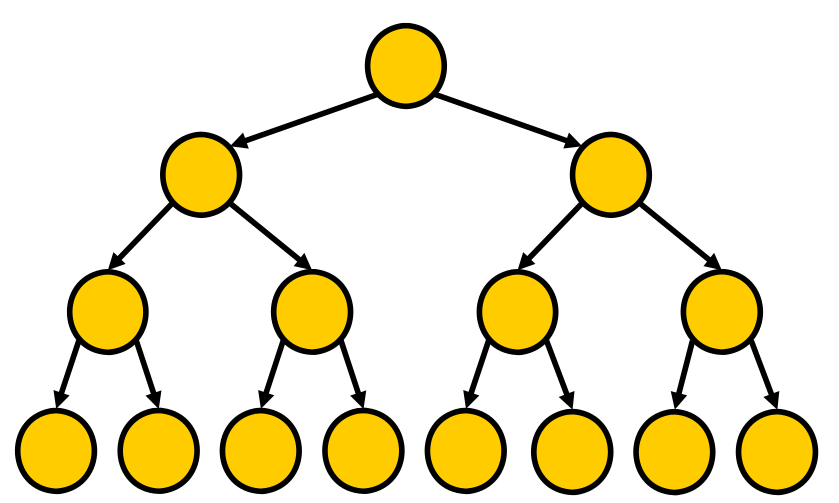
\includegraphics[width=0.25\linewidth]{fullbt}
  \end{tabular}
  \begin{tabular}{l}
    Complete BT \\
    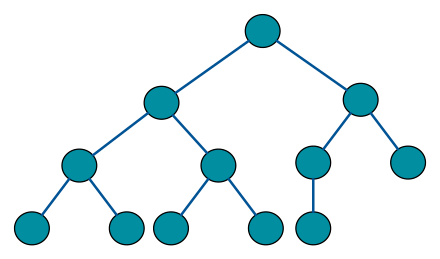
\includegraphics[width=0.25\linewidth]{completebt}
  \end{tabular}

  \begin{itemize}
    \item \textbf{Full} BT = every node has either 0 or 2 children
    \item \textbf{Complete} BT = Every level except the last is completely filled, and all nodes in the last level are as far left as possible
  \end{itemize}

  \subsubsection{Properties}
  \begin{itemize}
    \item \textbf{Full BT}: no of nodes = $N$ = $2^h - 1$, height = $\log(N+1)$
    \item \textbf{Complete BT}: max($N$) = $2^{h-1}$, min($N$) = $2^{h} - 1$
  \end{itemize}

  \subsubsection{BT Traversal}
  \begin{itemize}
    \item Post-order
    \item Pre-order
    \item In-order
    \item Level-order: Traverse the tree level by level from left to right. (BFS)
  \end{itemize}

  \subsection{BST}
  \textbf{Property}: All keys smaller then root in left subtree, larger in right subtree.\\
  Case of deleting node with 2 children: move smallest node in right subtree to the deleted node.
  %		\begin{minted}{javascript}

  %		\end{minted}
\end{multicols*}
\end{document}
